\documentclass[margin=0mm,tikz]{standalone}

\usepackage{tikz}
\usepackage{xcolor}
\usepackage{amsmath}

\usetikzlibrary{positioning}
\usetikzlibrary{fit}
\usetikzlibrary{calc}
\usetikzlibrary{arrows}
\usetikzlibrary{arrows.meta}
\usetikzlibrary{quotes}
\usetikzlibrary{backgrounds}

\pgfdeclarelayer{background}
\pgfsetlayers{background,main}

% -----------------------
% colors
% -----------------------
\definecolor{N2color}{RGB}{180, 203, 231}
\definecolor{N3color}{RGB}{172, 192, 231}
\definecolor{N202color}{RGB}{176, 198, 231}

\definecolor{polar1}{RGB}{180, 203, 231}
\definecolor{polar2}{RGB}{172, 192, 231}
\definecolor{equat1}{RGB}{231, 213, 168}
\definecolor{equat2}{RGB}{231, 203, 173}


% Set background color
%\pagecolor{white}


\tikzstyle{cface} = [
	very thick, 
	draw=black,
	top color=equat1,
	bottom color=equat1,
	minimum size=5cm,
]
\tikzstyle{n2face} = [
	very thick, 
	draw=black,
	top color=polar1,
	bottom color=polar1,
	minimum size=5cm,
	opacity=0.5
]
\tikzstyle{n3face} = [
	very thick, 
	draw=black,
	top color=polar2,
	bottom color=polar2,
	minimum size=5cm,
	opacity=0.5
]
\tikzstyle{diag} = [
	dotted,
	opacity=0.5
]
\tikzstyle{cell} = [
	draw,
	minimum size=1.825cm,
	%opacity=0.5
]

% Box with different colors, modified from
% https://tex.stackexchange.com/questions/343354/tikz-rectangle-with-diagonal-fill-two-colors
\tikzset{
	diagonal fill/.style 2 args={
		path picture={
			\fill[#1] (path picture bounding box.south) -| (path picture bounding box.north) -- cycle;
			\fill[#2] (path picture bounding box.north) -| (path picture bounding box.south) -- cycle;
		}
	},
}



\begin{document}
	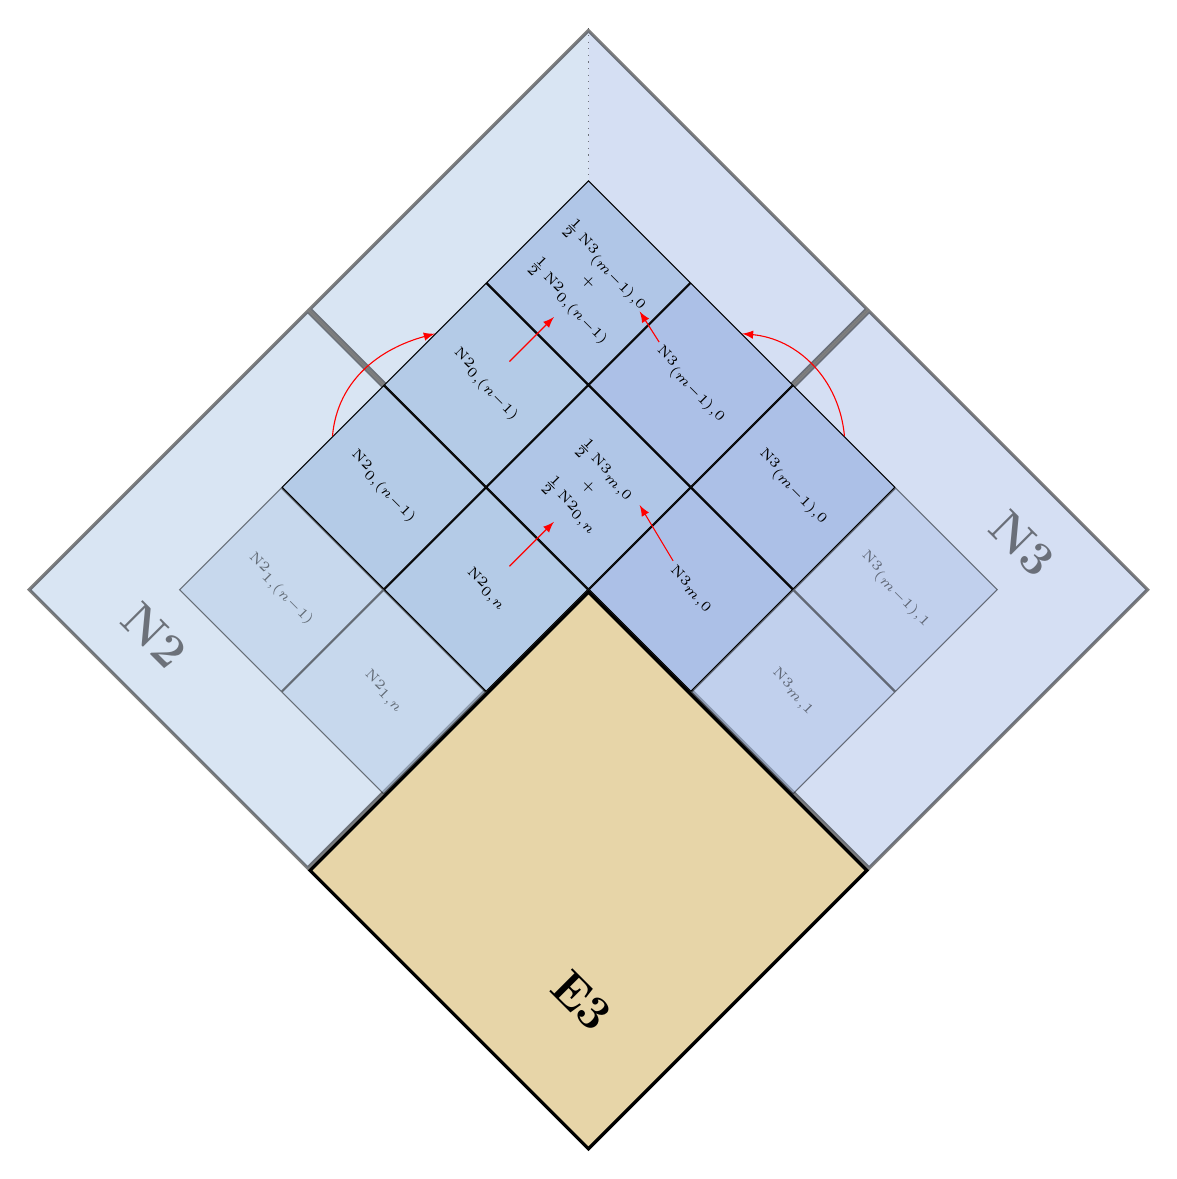
\begin{tikzpicture}[node distance=0cm and 0cm, rotate=-45, transform shape]
		
	%
	% North faces
	\node[cface, label={[label distance=-2.3cm]-90:\LARGE\textbf{E3}}] (E3) {};
	\node[n3face, above=of E3, label={[label distance=-3cm, opacity=0.5]0:\LARGE\textbf{N3}}] (N3) {};
	\node[diagonal fill={polar1}{polar2}, very thick, draw=black, minimum size=5cm, opacity=0.5, above left=of E3] (N202) {};
	\draw[diag] (N202.north west)--(N202.south east);
	\node[n2face, left=of E3, label={[label distance=-3cm, opacity=0.5]180:\LARGE\textbf{N2}}] (N2) {};
	
	%
	% Cells in N2
	\node[cell, anchor=north east, fill=N2color] at (N2.north east) (N2_0_n) {\tiny N2$_{0,n}$};
	\node[cell, left=of N2_0_n, fill=N2color] (N2_0_n-1) {\tiny N2$_{0,(n-1)}$};
	
	\node[cell, below=of N2_0_n, fill=N2color, opacity=0.5] (N2_1_n) {\tiny N2$_{1,n}$};
	\node[cell, below=of N2_0_n-1, fill=N2color, opacity=0.5] (N2_1_n-1) {\tiny N2$_{1,(n-1)}$};
	
	%
	% Cells in N3
	\node[cell, anchor=south west, fill=N3color] at (N3.south west) (N3_m_0) {\tiny N3$_{m,0}$};
	\node[cell, above=of N3_m_0, fill=N3color] (N3_m-1_0) {\tiny N3$_{(m-1),0}$};
	
	\node[cell, right=of N3_m_0, fill=N3color, opacity=0.5] (N3_m_1) {\tiny N3$_{m,1}$};
	\node[cell, right=of N3_m-1_0, fill=N3color, opacity=0.5] (N3_m-1_1) {\tiny N3$_{(m-1),1}$};
	
	%
	% Cells in N202
	\node[cell, left=of N3_m-1_0, fill=N3color, opacity=1.0] (N202_m-1_n) {\tiny $\operatorname{N3}_{(m-1), 0}$};
	
	\node[cell, above=of N2_0_n-1, fill=N2color, opacity=1.0] (N202_m_n-1) {\tiny $\operatorname{N2}_{0, (n-1)}$};
	
	\node[cell, above=of N2_0_n, fill=N202color] (N202_m_n) {\tiny \shortstack{$\frac{1}{2}\operatorname{N3}_{m,0}$\\$+$\\$\frac{1}{2}\operatorname{N2}_{0,n}$}};
	\node[cell, above left=of N202_m_n, fill=N202color] (N202_m-1_n-1) {\tiny \shortstack{$\frac{1}{2}\operatorname{N3}_{(m-1),0}$\\$+$\\$\frac{1}{2}\operatorname{N2}_{0,(n-1)}$}};
	
	%
	% Arrows
	
	% N2 to N202
	\draw[-latex, red] ([yshift=-0.5cm]N2_0_n.north) -- ([yshift=0.3cm]N202_m_n.south);
	\draw[-latex, red] ([yshift=-0.5cm]N202_m_n-1.north) -- ([yshift=0.3cm]N202_m-1_n-1.south);
	
	\draw[-latex, red] (N2_0_n-1.west) to[out=130,in=240] (N202_m_n-1.west);

	% N3 to N202
	\draw[-latex, red] ([xshift=0.5cm, yshift=0.1cm]N3_m_0.west) -- ([xshift=-0.3cm, yshift=0.3cm]N202_m_n.east);
	\draw[-latex, red] ([xshift=0.25cm, yshift=0.1cm]N202_m-1_n.west) -- ([xshift=-0.2cm, yshift=0.2cm]N202_m-1_n-1.east);
	
	\draw[-latex, red] (N3_m-1_0.north) to[out=140, in=40] (N202_m-1_n.north);
	
	\end{tikzpicture}
\end{document}